\documentclass[UTF8]{article} %article 文档
\usepackage{ctex}  %使用宏包(为了能够显示汉字)
\usepackage{lscape}
\usepackage{amsmath}
\usepackage{color}
\usepackage{amssymb}
\usepackage{cases}
\usepackage{float}
\usepackage{graphicx}
\usepackage{subcaption}
\usepackage{mathtools}
\usepackage{booktabs}
\usepackage{multirow}
\usepackage{calc}
\usepackage{arydshln}
\usepackage[hidelinks]{hyperref}
\usepackage{cite}
\usepackage{chngcntr}
\counterwithin{figure}{section}

\graphicspath{{image/}{figure/}{fig/}{img/}}

\title{机械部培训——零件篇}  %文章标题
\author{董仕豪,卢勇来}   %作者的名称
\date{\today}       %日期

% 设置页面的环境,a4纸张大小,左右上下边距信息
\usepackage[a4paper,left=15mm,right=15mm,top=25.4mm,bottom=25.4mm]{geometry}
\begin{document}
\maketitle          %添加这一句才能够显示标题等信息
%生成目录设置
\newpage
\tableofcontents

\newpage

\section{绪论}
机械零件(machine element)又称机械元件(machine part)是构成机械的基本元件,是组成机械和机器的不可分拆的单个制件。机械零件既是研究和设计各种设备中机械基础件的一门学科,也是零件和部件的泛称。本文档旨在为机械部入门的同学介绍常用的机械零件知识,为今后的机械设计提供一定的帮助。

\begin{figure}[h]
  \centering
  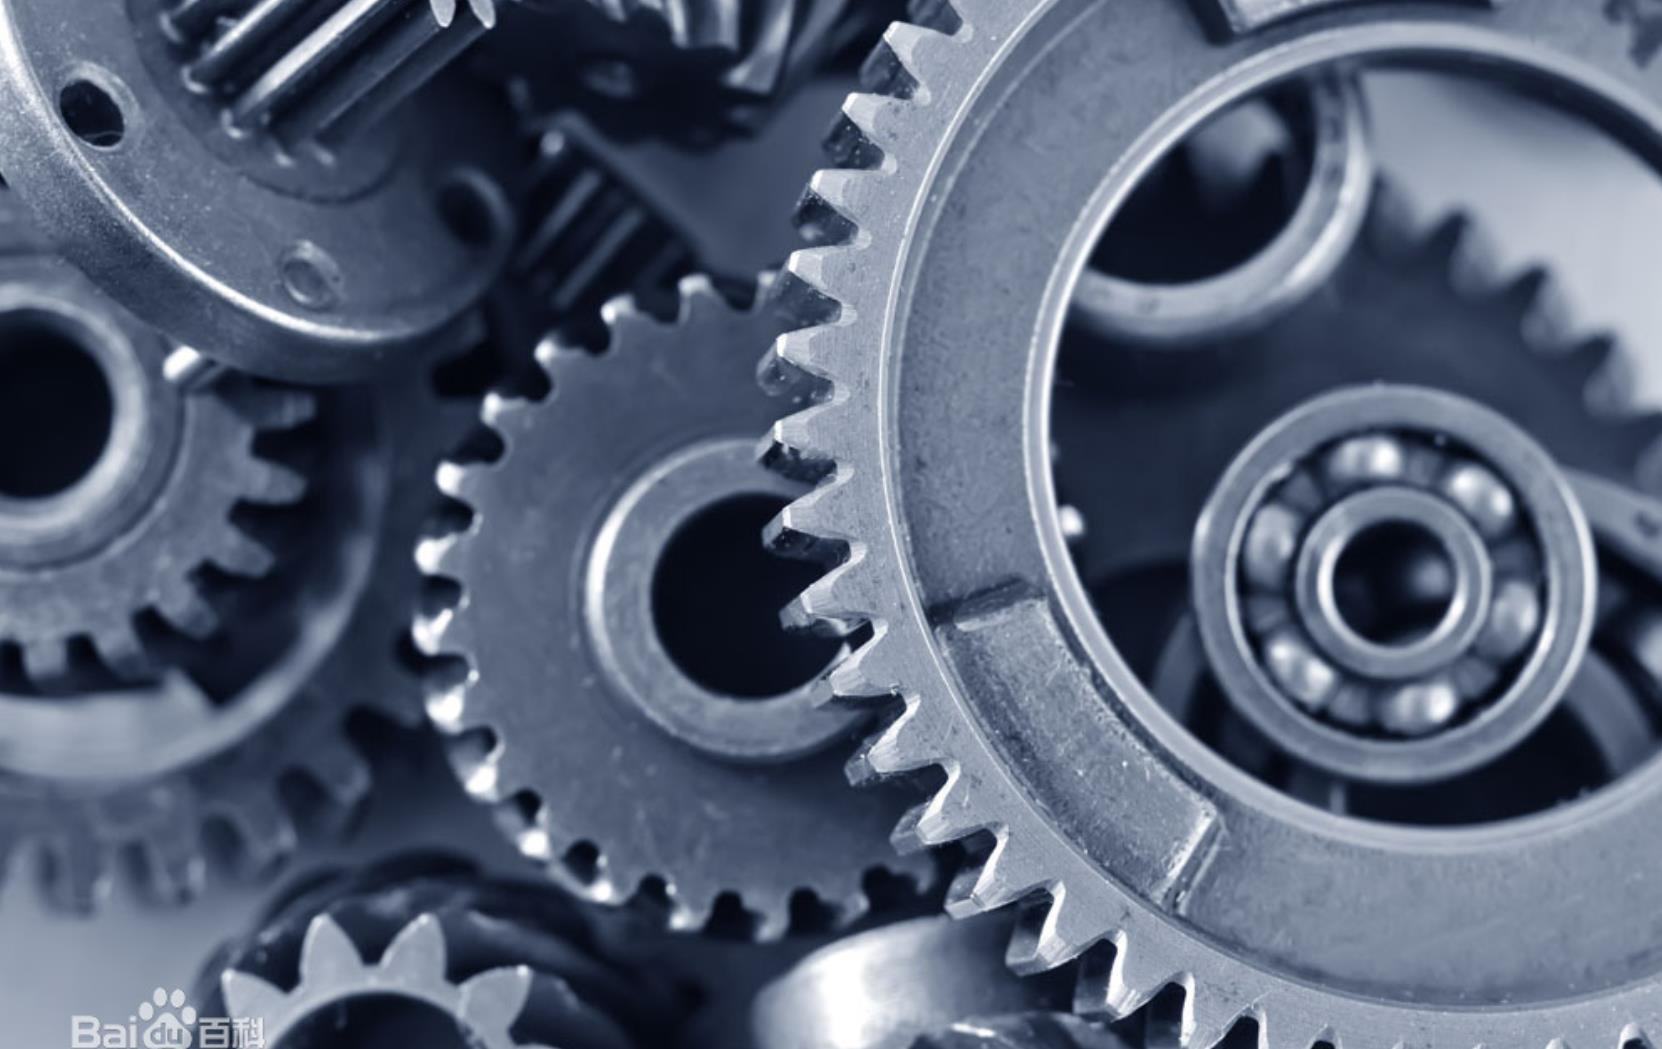
\includegraphics[width=0.5\textwidth]{kai1.jpg}
  \caption{机械零件}
  \label{fig:kai}
\end{figure}

\section{常用材料}
本章就机械设计中常用的材料进行讲解,介绍管材、板材等多种常用的工程材料。

\subsection{管材}
管材质量轻,强度刚度高,受力变形小,常用于支撑结构的设计,比如车架,保险杠等。管材在RM机器人设计当中,使用十分广泛,\textbf{几乎所有机器人骨架结构是由铝方管搭建而成},其中又以铝方管最为常用。

\begin{figure}[H]
  \centering
  \begin{subfigure}[b]{0.39\textwidth}
         \centering
         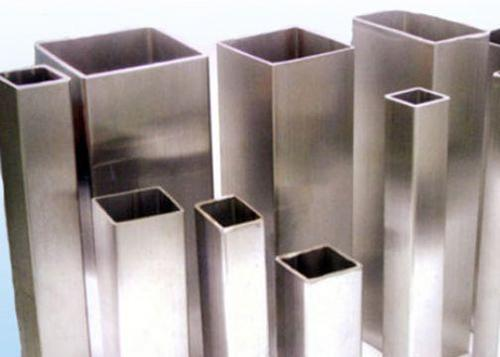
\includegraphics[width=\textwidth]{lv.png}
          \caption{铝方管}
          \label{f4}
  \end{subfigure}
  \quad
  \begin{subfigure}[b]{0.45\textwidth}
          \centering
          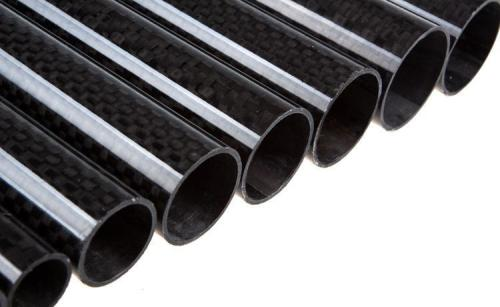
\includegraphics[width=\textwidth]{tan.png}
          \caption{碳管}
          \label{f5}
  \end{subfigure}
  \caption{常用管材 }
  \label{wg}
\end{figure}

\subsubsection{铝方管}
\begin{itemize}
  \item \textbf{简介:} 铝方管价格便宜,质量轻,加工精度较高,是车架设计最主要的材料。铝方管的加工方式主要有焊接,打孔,镂空。铝方管与铝方管之间可以进行焊接也可以通过螺栓连接,铝方管与其他零件的连接主要通过螺栓连接,所以铝方管设计主要以设计孔位为主。另外铝方管加工孔位一般为正偏差,螺栓穿过较为容易,不需要留尺寸余量。镂空主要用于轻量化设计,镂空时需要进行仿真分析,保证强度。
  \item \textbf{规格介绍:} 铝方管规格一般表示为长 $\times$ 宽 $\times$ 壁厚。单位默认mm,比如$20 \times 20 \times 1$表示截面长宽均为20mm,壁厚为1mm的铝方管。队内根据强度需求选用壁厚1-3mm的铝方管。
  
  \begin{figure}[h]
    \centering
    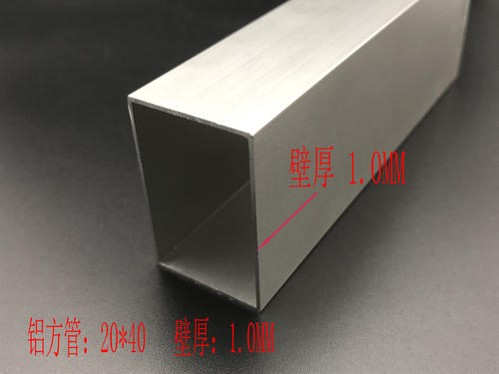
\includegraphics[width=0.3\textwidth]{chicun1.jpg}
    \caption{某公司铝方管尺寸规格}
  \end{figure}

  \item \textbf{注意事项:} 
  
  \begin{itemize}
    \item 同等横截面积(保持质量不变),越粗的铝方管(壁厚小)强度越高。所以增加强度\textbf{优先考虑选用更粗的铝方管},其次考虑增加厚度。
    \item 为增加铝方管抗压性能,可以在管内进行填充(如亚克力,机加工内衬件等)
    \item 因为铝方管中空,安装螺栓时用力过大会导致表面凹陷,所以\textbf{安装贯穿铝方管的螺栓时需加垫片},且不可用力过度。
  \end{itemize}
\end{itemize}

\subsubsection{碳管}

\begin{itemize}
  \item \textbf{简介:} 碳方管相比于铝方管碳管质量更轻,强度更高,但是加工困难,价格较高。一般只在轻量化设计时代替铝方管使用。碳圆管价格较低,使用较多。
  碳方管设计除不能焊接外与铝方管类似,碳圆管一般只能购买特定规格使用。

  \item \textbf{规格介绍:} 碳方管规格同样表示为长$\times$宽$\times$壁厚。碳圆管规格一般表示为内径$\times$外径。队内碳圆管使用较多,方管很少使用。

  \begin{figure}[H]
    \centering
    \begin{subfigure}[b]{0.39\textwidth}
           \centering
           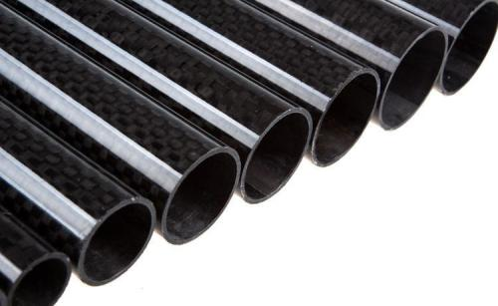
\includegraphics[width=\textwidth]{tan1.png}
            \caption{圆形碳管}
    \end{subfigure}
    \quad
    \begin{subfigure}[b]{0.3\textwidth}
            \centering
            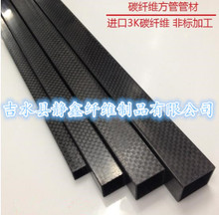
\includegraphics[width=\textwidth]{tan2.png}
            \caption{方形碳管}
    \end{subfigure}
    \caption{碳管分类}
  \end{figure}

  \item \textbf{注意事项:} 碳管有哑光和亮光之分,哑光碳管表面粗糙度大,无法配合直线轴承使用。

\end{itemize}

\subsubsection{型材}
\begin{itemize}
  \item \textbf{简介:} 型材具有设计灵活,装配方便的特点,但是型材质量大,装配精度低,一般不作为机器人构建材料,\textbf{而用于搭建场地或是测试机构}。型材为标准件,购买相应规格的型材使用。安装需要搭配船型螺母和角码。


  \item \textbf{规格介绍:} 铝型材规格一般表示为长$\times$宽。

  \begin{figure}[H]
    \centering
    \begin{subfigure}[b]{0.39\textwidth}
           \centering
           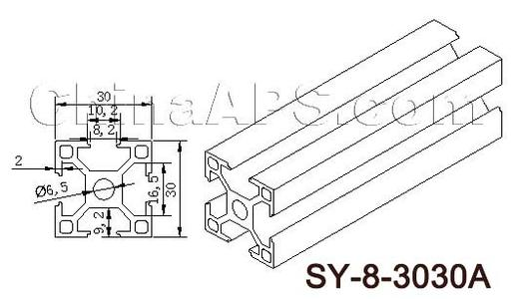
\includegraphics[width=\textwidth]{xing1.png}
            \caption{型材截面形状}
    \end{subfigure}
    \quad
    \begin{subfigure}[b]{0.4\textwidth}
            \centering
            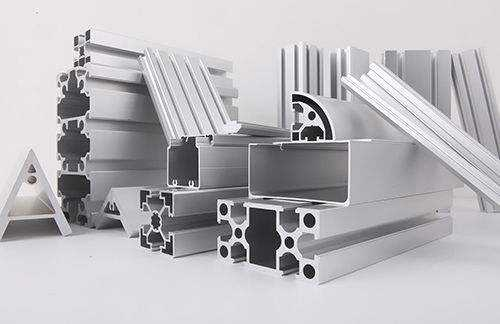
\includegraphics[width=\textwidth]{xing2.png}
            \caption{各种型材}
    \end{subfigure}
    \caption{型材}
  \end{figure}

  \item \textbf{注意事项:} 在型材上固定的螺母为船型螺母,而船型螺母没有防松功能,容易松。
  \item \textbf{安装实例:} 如图\ref{xing}所示为型材螺母安装示意图,中间图为角码安装实例。另外,型材角码具有多种类型,使用不同类型的角码,可以将型材组合成任意形状,且安装和拆卸都十分方便,可重复多次使用,使用方式自由多变。
  \begin{figure}[H]
    \centering
    \begin{subfigure}[b]{0.3\textwidth}
           \centering
           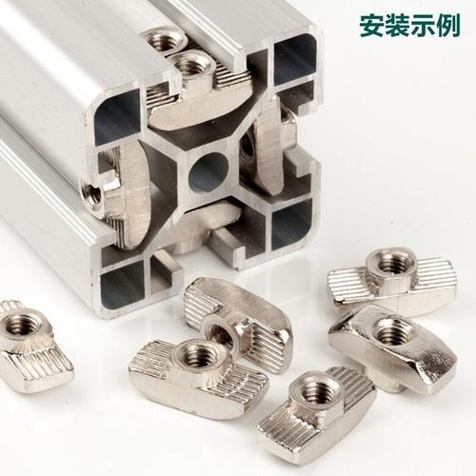
\includegraphics[width=\textwidth]{chuan1.png}
            \caption{船型螺母安装示例}
    \end{subfigure}
    \quad
    \begin{subfigure}[b]{0.3\textwidth}
            \centering
            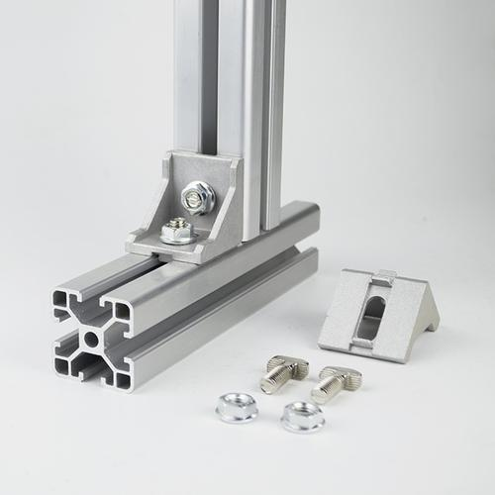
\includegraphics[width=\textwidth]{chaun2.png}
            \caption{角码安装示例}
    \end{subfigure}
    \begin{subfigure}[b]{0.3\textwidth}
      \centering
      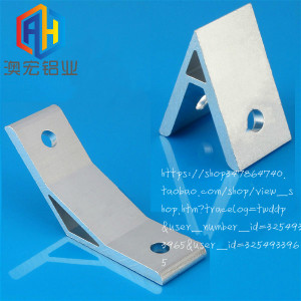
\includegraphics[width=\textwidth]{chaun3.png}
      \caption{其他角码}
    \end{subfigure}
    \caption{型材安装示例}
    \label{xing}
  \end{figure}
\end{itemize}

\subsection{板材}
板材加工方便,形状设计自由多变,常用于各种元件的安装件,支撑件设计。板材在RM机器人设计当中应用也相当广泛,板材零件由于具备加工方便,设计自由的优势,是机器人结构设计当中的优先选择。板材零件配合直角连接件,能够完成绝大部分结构的设计要求。

\subsubsection{碳板}

\begin{itemize}
  \item \textbf{简介:} 碳板强度高,质量轻,加工精度高,\textbf{是机器人各种安装件支撑件设计的主要材料}。板材设计为平面设计,先设计相应安装孔位,在设计外部轮廓,最后根据强度需要进行适当镂空。

  \item \textbf{规格介绍:} 碳板材规格一般表示板厚。队内使用碳板厚度从$1mm$到$8mm$不等。一般情况下使用$4mm$碳板,不受力且无刚度要求可用$1mm$;不受力或受力较小($10kg$量级)结构可用$2mm$;正常受力($100kg$量级)用$4mm$;受力较大或刚度要求高或受大冲击可用$8mm$。

  
  \begin{figure}[h]
    \centering
    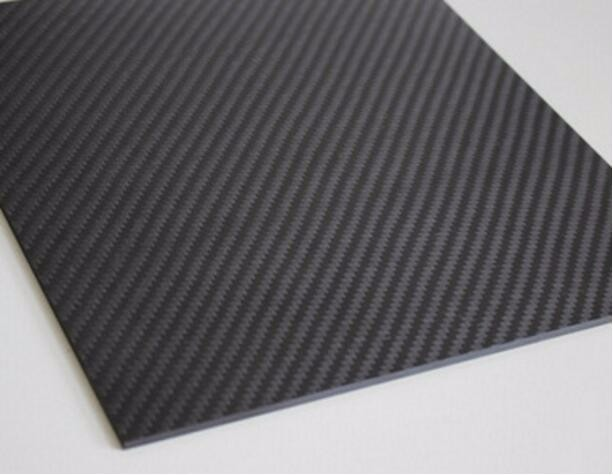
\includegraphics[width=0.3\textwidth]{ban1.png}
    \caption{碳板}
  \end{figure}

  \item \textbf{注意事项:} 
  
  \begin{itemize}
    \item 碳板孔位加工精度误差一般为负偏差($-0.1mm$左右),精度要求较小时建议尺寸设计时留好余量,比如m4的螺栓孔设计尺寸为$4.1mm$,可以减少装配时间。
    \item 板材设计所有角都要倒圆角,防止应力集中。	
  \end{itemize}
  
\end{itemize}

\subsubsection{玻纤板}

\begin{itemize}
  \item \textbf{简介:}   玻纤板强度略低于碳板,质量略重于碳板,但是价格便宜。常用于构建机器人测试版。经费不足时,也用于最终产品。玻纤板与碳板完全可以相互替代使用,且性能相差较小,是碳板的下位替代。

  \item \textbf{规格介绍:} 同碳板。

  \begin{figure}[h]
    \centering
    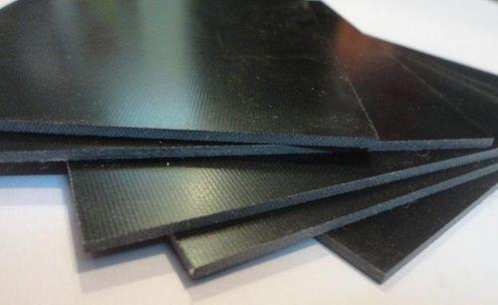
\includegraphics[width=0.3\textwidth]{ban2.png}
    \caption{玻纤板}
  \end{figure}

\end{itemize}

\subsubsection{亚克力板}

\begin{itemize}
  \item \textbf{简介:} 亚克力板价格低廉,加工方便。常用于各种测试结构搭建。但是亚克力板强度低,一般不用于最终产品的搭建。亚克力加工周期短(工训提供激光切割),价格低廉,广泛用于研发测试阶段。一般亚克力实际厚度偏小,且加工孔位误差大致有$+0.1mm$左右(激光光束宽度造成),故装配时会有较大间隙。
  \item \textbf{规格介绍:} 同碳板。
  
  \begin{figure}[h]
    \centering
    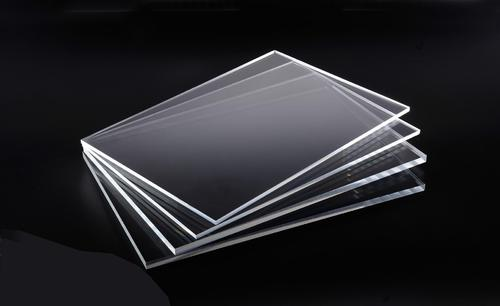
\includegraphics[width=0.3\textwidth]{ban3.png}
    \caption{亚克力板}
  \end{figure}

\end{itemize}

\subsubsection{机加工件}

\begin{itemize}
  \item \textbf{简介:} 机加工件为立体结构设计,比板材设计更为灵活,部分板材设计不方便实现的结构可以考虑设计机加工件。另外机加工件可以设计螺纹孔,可以解决部分螺栓装配困难的问题。机加工件常规加工方式主要有线切割,车,铣,打孔等。机加工件设计灵活,\textbf{设计时需要考虑加工工艺},避免出现无法加工的结构。虽然机加工件成本较高,但使用得当,可以显著简化结构。

  \item \textbf{注意事项:} 机加工件关键尺寸需要标注误差要求,比如轴与孔配合,孔需要标注正偏差,轴标注负偏差。没有标注偏差要求的尺寸一般默认没有误差要求,加工得到的零件可能会出现无法安装的情况。

  
  \begin{figure}[h]
    \centering
    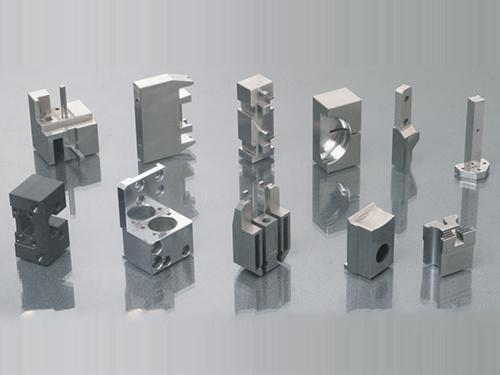
\includegraphics[width=0.3\textwidth]{ji.png}
    \caption{机加工零件}
  \end{figure}

\end{itemize}

\subsubsection{3D打印件}

\begin{itemize}
  \item \textbf{简介:} 3D打印(3DP)即快速成型技术的一种,又称增材制造 ,它是一种以数字模型文件为基础,运用粉末状金属或塑料等可粘合材料,通过逐层打印的方式来构造物体的技术。3D打印件可以设计任意形状,不用考虑加工工艺的问题,经常作为研发测试用件。
  
  \begin{figure}[h]
    \centering
    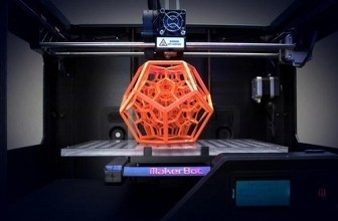
\includegraphics[width=0.3\textwidth]{3.png}
    \caption{3D打印}
  \end{figure}

  \item \textbf{注意事项:} 
  \begin{itemize}
    \item 3D打印件\textbf{强度较低},不能作为承力结构。
    \item 表面粗糙度较差,可以用抛光液适当改善。
    \item 3D打印件一般\textbf{尺寸偏大},大约有$0.5mm$的正偏差,可以在设计是预留尺寸余量。

  \end{itemize}

\end{itemize}

\section{连接零件}
本章主要介绍用于连接的零(部)件,如螺纹联接、楔联接、销联接、键联接、花键联接、过盈配合联接、弹性环联接、铆接、焊接和胶接等。
\subsection{螺栓螺母}
螺栓螺母配合使用,用于\textbf{紧固连接两个带有通孔的零件}。螺栓的型号表示: \textbf{M-圆径*长度(CM)},即 M-数字号。M 代表米制螺纹,比如 $M8*1.25*50$ 意思是公称直径为 $8mm$ 螺距为 $1.25$ 螺杆长度为 $50mm$,L 表示螺栓的长度,D 表示公称直径。螺栓性能等级分3.6、4.6、4.8、5.6、6.8、8.8、9.8、10.9、12.9等10余个等级,强度等级所谓8.8级和10.9级是指螺栓的抗剪切应力等级为$8.8GPa$和$10.9GPa$。\textbf{队内一般情况选用圆柱头内六角螺钉。型号主要以M3,M4,M5为主。}搭配内六角扳手方便拆卸,螺母一般选用防松螺母,注意:

\begin{itemize}
  \item 螺栓干涉,包括螺栓头,螺母干涉;装配干涉(没有给工具预留空间);螺栓头干涉问题是设计过程中十分容易忽略的问题,最好在图上安装螺栓,避免干涉问题。
	\item 螺栓安装时注意合适的拧紧力矩,拧紧力矩不足会导致连接产生间隙,拧紧力矩过大则会导致滑丝或者破坏零件。
  \item 必须要考虑防松问题,包括(不限于)防松螺母,螺丝胶等方式。
\end{itemize}

常见的螺栓螺母类型有以下几种:
\begin{itemize}
  \item \textbf{沉头螺栓:}螺栓头可沉入零件内部,一般在螺栓头易发生干涉情况下使用。使用时需要在零件上加工沉头孔。
  
  \begin{figure}[H]
    \centering
    \begin{subfigure}[b]{0.39\textwidth}
           \centering
           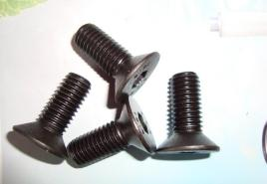
\includegraphics[width=\textwidth]{luo1.png}
            \caption{沉头螺栓}
    \end{subfigure}
    \quad
    \begin{subfigure}[b]{0.3\textwidth}
            \centering
            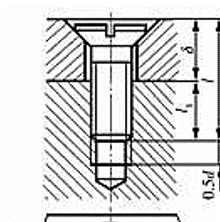
\includegraphics[width=\textwidth]{luo11.png}
            \caption{沉头螺栓安装方式}
    \end{subfigure}
    \caption{沉头螺栓示意图}
  \end{figure}

	\item \textbf{紧定螺栓:}专供固定机件相对位置用的一种螺钉,一般用于电机轴与法兰直接的固定。紧定螺栓容易滑丝。使用时注意拧紧力矩不宜过大。

  \begin{figure}[H]
    \centering
    \begin{subfigure}[b]{0.39\textwidth}
           \centering
           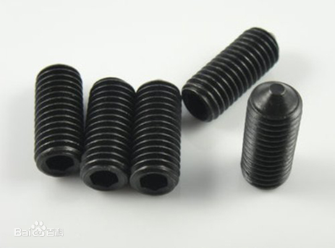
\includegraphics[width=\textwidth]{luo2.png}
            \caption{紧定螺栓}
    \end{subfigure}
    \quad
    \begin{subfigure}[b]{0.4\textwidth}
            \centering
            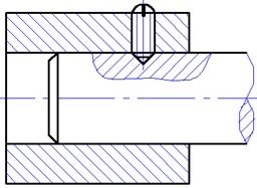
\includegraphics[width=\textwidth]{luo22.png}
            \caption{紧定螺栓安装方式}
    \end{subfigure}
    \caption{紧定螺栓示意图}
  \end{figure}

  \item \textbf{轴肩螺栓:}轴肩螺钉也叫塞打螺丝。 是在螺丝靠近冒头处有一段没有螺纹的柱体,安装后柱体部分可以作为轴或其它功能使用。队内一般配合轴承使用,实现铰链接。
  
  \begin{figure}[h]
    \centering
    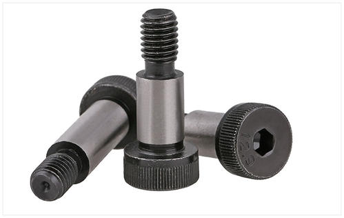
\includegraphics[width=0.25\textwidth]{luo3.png}
    \caption{轴肩螺栓}
  \end{figure}

  \item \textbf{子母螺栓:}子母螺丝是由子钉和母钉构成的螺丝。可以避免螺母干涉的情况。
  
  \begin{figure}[h]
    \centering
    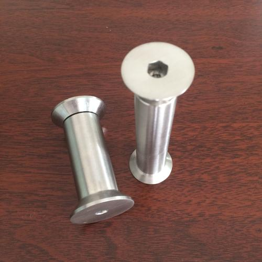
\includegraphics[width=0.25\textwidth]{luo4.png}
    \caption{子母螺栓}
  \end{figure}

  \item \textbf{手拧螺栓:}可以直接用手拧紧的螺栓,用于需要经常拆卸的场合。
  
  \begin{figure}[h]
    \centering
    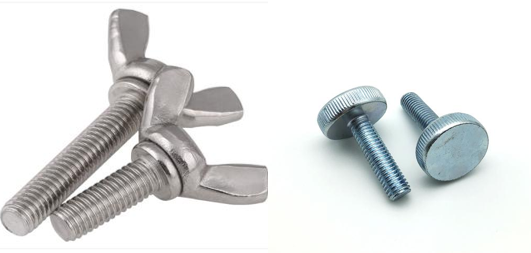
\includegraphics[width=0.25\textwidth]{luo5.png}
    \caption{手拧螺栓}
  \end{figure}

  \item \textbf{自攻螺丝:}自攻螺丝用于非金属或木材,可以不用打底孔和攻牙直接旋进去。常用于木工连接,队内场地搭建使用较多。
  
  \begin{figure}[h]
    \centering
    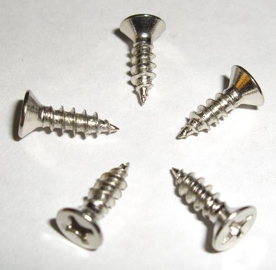
\includegraphics[width=0.25\textwidth]{luo6.png}
    \caption{自攻螺丝}
  \end{figure}

\end{itemize}

\subsection{角码}
角码是连接90度直角相交构件的连接件。常用于两板之间的直角连接。角码种类较多,根据需要选用不同的角码进行连接。队内一般使用直角转接件进行直角连接。另外型材角码用于型材之间的装配
\begin{figure}[H]
  \centering
  \begin{subfigure}[b]{0.3\textwidth}
         \centering
         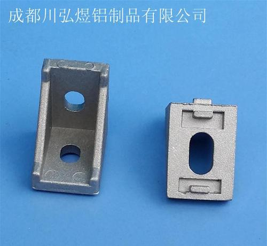
\includegraphics[width=\textwidth]{jiao1.png}
          \caption{型材角码}
  \end{subfigure}
  \quad
  \begin{subfigure}[b]{0.4\textwidth}
          \centering
          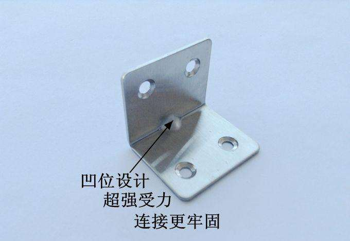
\includegraphics[width=\textwidth]{jiao2.png}
          \caption{普通角码}
  \end{subfigure}
  \quad
  \begin{subfigure}[b]{0.3\textwidth}
    \centering
    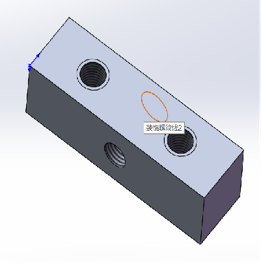
\includegraphics[width=\textwidth]{jiao3.png}
    \caption{直角转接件}
\end{subfigure}
\quad
\begin{subfigure}[b]{0.4\textwidth}
  \centering
  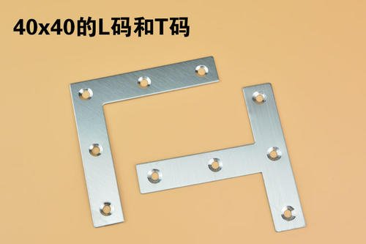
\includegraphics[width=\textwidth]{jiao4.png}
  \caption{其他角码}
\end{subfigure}
  \caption{角码示意图示意图}
\end{figure}

\subsection{法兰}
法兰是轴与平面或轴与轴之间相互连接的零件。比如电机轴与轮毂之间的连接。根据需要选用不同类型的法兰。队内常用3508电机法兰用于电机轴与麦轮之间的连接。
\begin{figure}[H]
  \centering
  \begin{subfigure}[b]{0.2\textwidth}
         \centering
         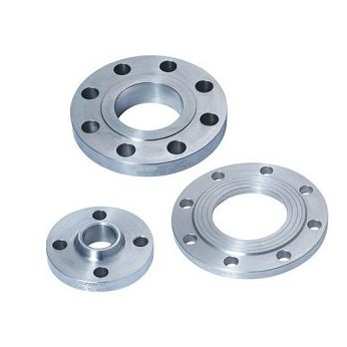
\includegraphics[width=\textwidth]{fa1.png}
          \caption{法兰}
  \end{subfigure}
  \quad
  \begin{subfigure}[b]{0.2\textwidth}
          \centering
          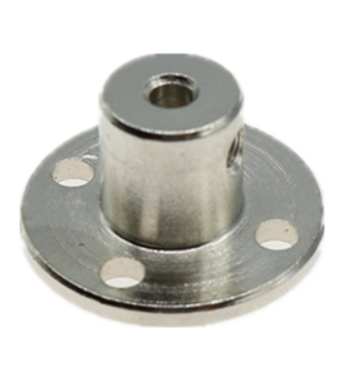
\includegraphics[width=\textwidth]{fa2.png}
          \caption{法兰盘}
  \end{subfigure}
  \begin{subfigure}[b]{0.3\textwidth}
    \centering
    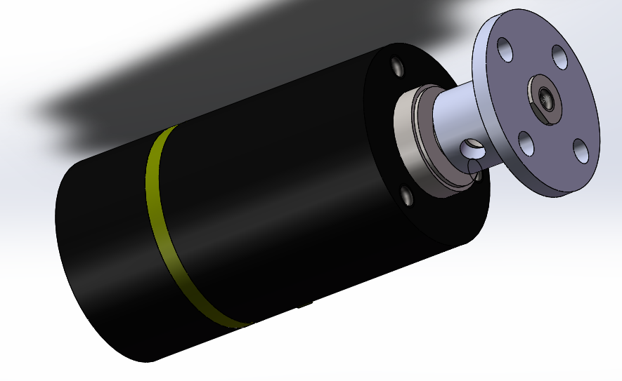
\includegraphics[width=\textwidth]{fa3.png}
    \caption{电机法兰示意图}
\end{subfigure}
  \caption{法兰示意图}
\end{figure}

\subsection{联轴器}
联轴器是指联接两轴或轴与回转件,在传递运动和动力过程中一同回转,在正常情况下不脱开的一种装置。常用的联轴器大多已标准化或规格化,一般情况下只需要正确选择联轴器的类型、确定联轴器的型号及尺寸。

\begin{figure}[H]
  \centering
  \begin{subfigure}[b]{0.25\textwidth}
         \centering
         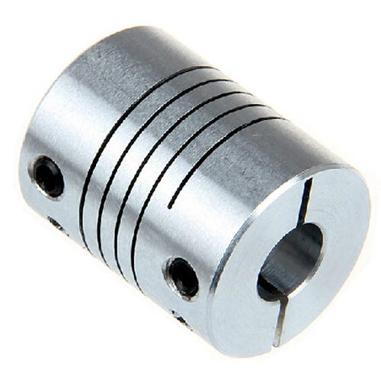
\includegraphics[width=\textwidth]{lian1.png}
          \caption{梅花联轴器}
  \end{subfigure}
  \quad
  \begin{subfigure}[b]{0.3\textwidth}
          \centering
          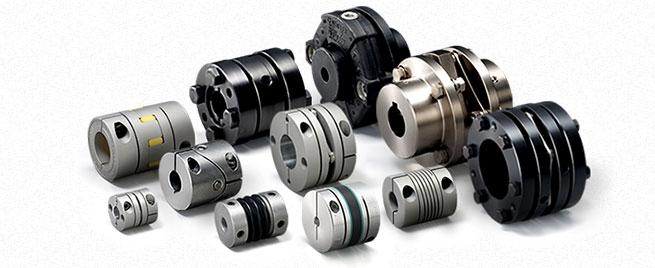
\includegraphics[width=\textwidth]{lian2.png}
          \caption{联轴器}
  \end{subfigure}
  \caption{联轴器示意图}
\end{figure}

\subsection{铰链}
铰链又称合页,是用来连接两个固体并允许两者之间做相对转动的机械装置。铰链种类主要有一般合页、弹簧铰链、液压缓冲铰链,可以根据需要选择铰链类型。

\begin{figure}[H]
  \centering
  \begin{subfigure}[b]{0.3\textwidth}
         \centering
         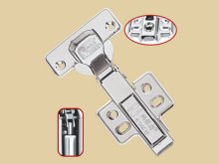
\includegraphics[width=\textwidth]{jl1.png}
          \caption{液压铰链}
  \end{subfigure}
  \quad
  \begin{subfigure}[b]{0.25\textwidth}
          \centering
          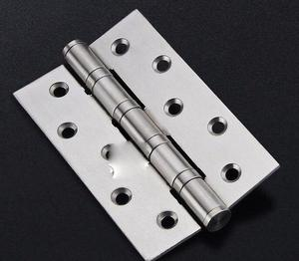
\includegraphics[width=\textwidth]{jl2.png}
          \caption{合页}
  \end{subfigure}
  \caption{铰链示意图}
\end{figure}

\subsection{销连接}
销是标准件,可用来作为定位零件,用以确定零件间的相互位置;也可起联接作用,以传递横向力或转矩;或作为安全装置中的过载切断零件。常用的销有圆柱销、圆锥销和开口销等。

\begin{figure}[H]
  \centering
  \begin{subfigure}[b]{0.35\textwidth}
         \centering
         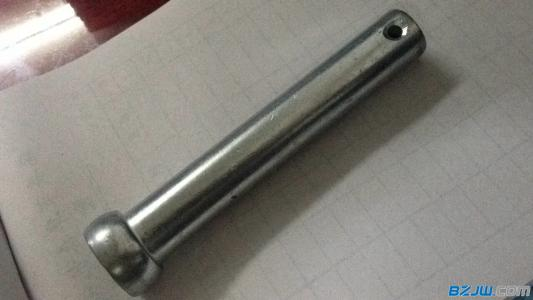
\includegraphics[width=\textwidth]{xiao1.png}
          \caption{销}
  \end{subfigure}
  \quad
  \begin{subfigure}[b]{0.4\textwidth}
          \centering
          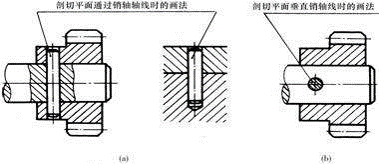
\includegraphics[width=\textwidth]{xiao2.png}
          \caption{连接示意图}
  \end{subfigure}
  \caption{销接示意图}
\end{figure}

\subsection{键连接}
键连接是通过键实现轴和轴上零件间的周向固定以传递运动和转矩。其中,有些类型还可以实现轴向固定和传递轴向力,有些类型并能实现轴向动联接。键连接可分为平键连接、半圆键连接、楔键连接和切向键连接。键的选择包括类型选择和尺寸选择两个方面。

选择键连接类型时,一般需考虑传递转矩大小,轴上零件沿轴向是否有移动及移动距离大小,对中性要求和键在轴上的位置等因素,并结合各种键连接的特点加以分析选择。事实上大部分情况下轴类零件传递扭矩是通过各种类型的键实现。因为键连接可以保证同轴度,而且可以消除间隙。而D形轴同轴性和精度均无法保证,方轴在设计当中更是不被允许

\begin{figure}[h]
  \centering
  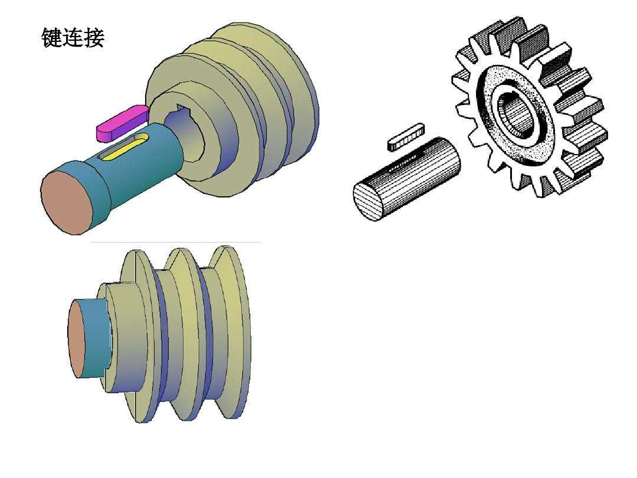
\includegraphics[width=0.3\textwidth]{jian1.png}
  \caption{键连接示意图}
\end{figure}


\subsection{铆接}

铆钉联接是利用铆钉将两个或两个以上的元件(一般为板材或型材)联接在一起的一种不可拆卸的静联接,简称铆接。铆钉有空心和实心两大类。最常用的铆接是实心铆钉联接。实心铆钉联接多用于受力大的金属零件的联接,空心铆钉联接用于受力较小的薄板或非金属零件的联接。

\begin{figure}[h]
  \centering
  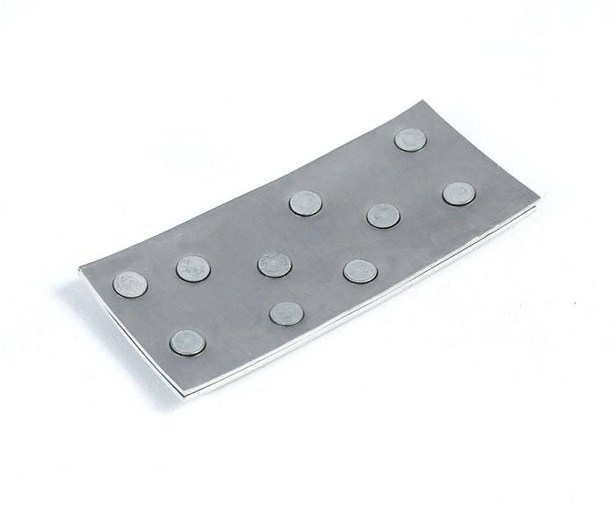
\includegraphics[width=0.3\textwidth]{mao1.png}
  \caption{铆接示意图}
\end{figure}

铆接分冷铆和热铆两种。热铆紧密性较好,但铆杆与钉孔间有间隙,不能参与传力。冷铆时钉杆镦粗,账满钉孔,钉杆与钉孔间无间隙。

铆接分类:
\begin{itemize}
  \item  \textbf{活动铆接:}结合件可以相互转动。不是刚性连接。如:剪刀,钳子。
  \item  \textbf{固定铆接:}结合件不能相互活动。这是刚性连接。如:角尺、三环锁上的铭牌、桥梁建筑。
  \item  \textbf{密封铆接:}铆缝严密,不漏气体、液体。这是刚性连接。
\end{itemize}

\textbf{抽芯铆钉:}抽芯铆钉(blind rivets) 、铆体(rivet body) 、钉芯(rivet stem or rivet mandrel )。是一类单面铆接用的铆钉,但须使用专用工具————拉铆枪(手动、电动、气动)进行铆接。铆接时,铆钉钉芯由专用铆枪拉动,使铆体膨胀,起到铆接作用.这类铆钉特别适用于不便采用普通铆钉(须从两面进行铆接)的铆接场合,故广泛用于建筑、汽车、船舶、飞机、机器、电器、家具等产品上。其中以开口型扁圆头抽芯铆钉应用最广,沉头抽芯铆钉适用于表面需要平滑的铆接场合,封闭型抽芯铆钉适用于要求较高载荷和具有一定密封性能的铆接场合。

\begin{figure}[H]
  \centering
  \begin{subfigure}[b]{0.3\textwidth}
         \centering
         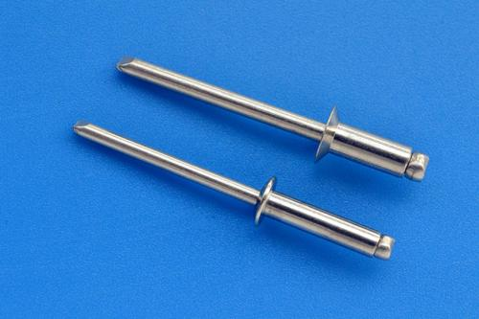
\includegraphics[width=\textwidth]{mao2.png}
          \caption{抽芯铆钉}
  \end{subfigure}
  \quad
  \begin{subfigure}[b]{0.3\textwidth}
          \centering
          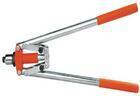
\includegraphics[width=\textwidth]{mao3.png}
          \caption{手动铆钉枪}
  \end{subfigure}
  \begin{subfigure}[b]{0.5\textwidth}
    \centering
    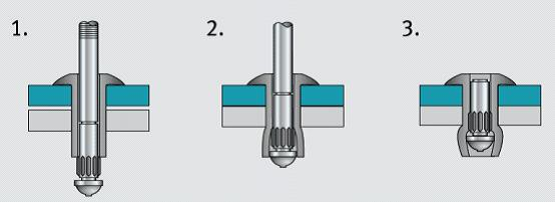
\includegraphics[width=\textwidth]{mao4.png}
    \caption{抽芯铆钉原理图}
  \end{subfigure}
  \caption{铆接示意图}
\end{figure}

\section{轴承}
轴承(Bearing)是当代机械设备中一种重要零部件。它的主要功能是支撑机械旋转体,降低其运动过程中的摩擦系数(friction coefficient),并保证其回转精度(accuracy)。

\subsection{深沟球轴承}

深沟球轴承是最具代表性的滚动轴承。与尺寸相同的其它类型轴承相比,该类轴承摩擦系数小,极限转速高,结构简单,制造成本低,精度高,无需经常维护,而且尺寸范围大、形式多,是应用最广的一类轴承。它主要承受径向载荷,也可承受一定的轴向载荷。当其仅承受径向载荷时,接触角为零。

深沟球轴承装在轴上后,在轴承的轴向游隙范围内,可限制轴或外壳两个方向的轴向位移,因此可在双向作轴向定位。当深沟球轴承具有较大的径向游隙时,具有角接触轴承的性能,可承受较大的轴向载荷 。在轴向载荷很大的高速运转工况下,深沟球轴承比推力球轴承更有优越性。此外,该类轴承还具有一定的调心能力,当相对于外壳孔倾斜2′~10′ 时,仍能正常工作,但对轴承寿命有一定影响。

\begin{figure}[H]
  \centering
  \begin{subfigure}[b]{0.4\textwidth}
         \centering
         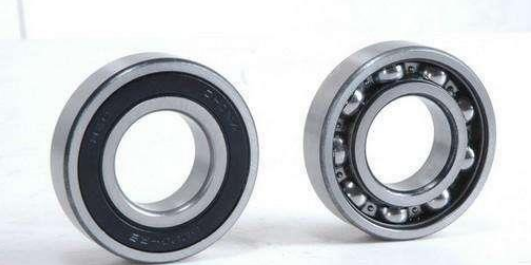
\includegraphics[width=\textwidth]{zhou1.png}
          \caption{深沟球轴承}
  \end{subfigure}
  \quad
  \begin{subfigure}[b]{0.2\textwidth}
          \centering
          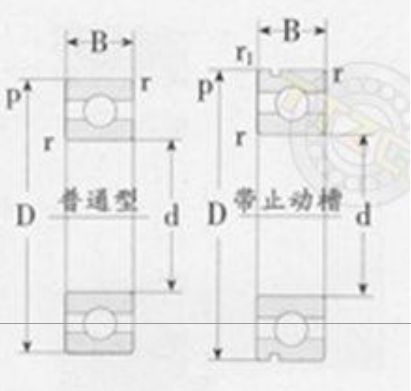
\includegraphics[width=\textwidth]{zhou2.png}
          \caption{深沟球轴承剖面图}
  \end{subfigure}
  \caption{深沟球轴承示意图}
\end{figure}

\subsection{法兰轴承}
法兰轴承外轮上带有凸缘法兰。特点是能简化主机结构,缩小主机尺寸,使轴承更容易定位。由于法兰轴承自带轴向定位结构,故在RM机器人设计当中应用十分广泛。

\begin{figure}[H]
  \centering
  \begin{subfigure}[b]{0.3\textwidth}
         \centering
         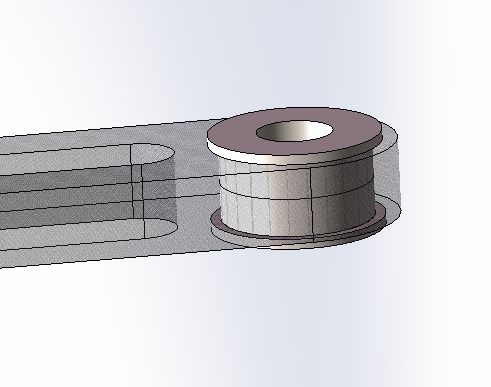
\includegraphics[width=\textwidth]{zhou3.png}
          \caption{法兰轴承使用实例}
  \end{subfigure}
  \quad
  \begin{subfigure}[b]{0.3\textwidth}
          \centering
          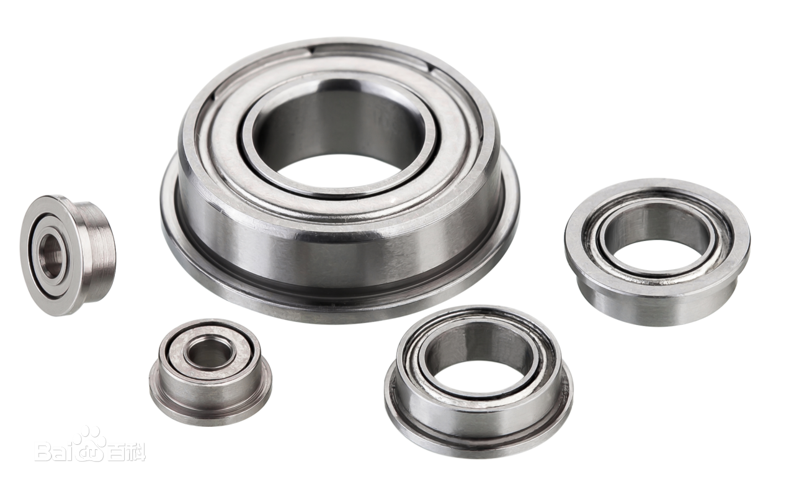
\includegraphics[width=\textwidth]{zhou4.png}
          \caption{法兰轴承}
  \end{subfigure}
  \caption{法兰轴承示意图}
\end{figure}

\subsection{推力球轴承}
推力球轴承分为单向和双向两种。 它们只能承受轴向载荷,绝不能承受任何径向载荷。推力轴承分紧圈和活圈两部分。紧圈与轴套紧,活圈支承在轴承座上。

按受力情况分单向推力球轴承和双向推力球轴承。单向推力球轴承,可承受单向轴向负荷。双向推力球轴承,可承受双向轴向负荷,其中轴圈与轴配合。座圈的安装面呈球面的轴承,具有调心性能,可以减少安装误差的影响。推力球轴承不能承受径向负荷,极限转速较低。

\begin{figure}[h]
  \centering
  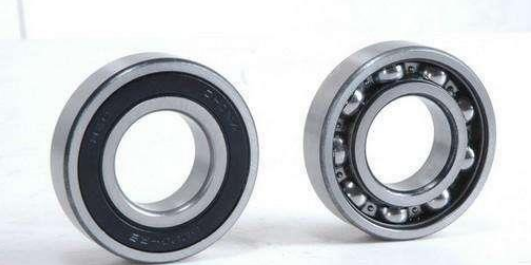
\includegraphics[width=0.3\textwidth]{zhou1.png}
  \caption{推力球轴承示意图}
\end{figure}

\subsection{直线轴承}
直线轴承是一种直线运动系统,用于直线行程与圆柱轴配合使用。由于承载球与轴承外套点接触,钢球以最小的摩擦阻力滚动,因此直线轴承具有摩擦小,且比较稳定,不随轴承速度而变化,能获得灵敏度高、精度高的平稳直线运动。直线轴承消耗也有其局限性,最主要的是轴承冲击载荷能力较差,且承载能力也较差,其次直线轴承在高速运动时振动和噪声较大。

注意,直线轴承对轴的光滑度和硬度要求较高,故直线轴承一般需配合钢轴使用。

\begin{figure}[H]
  \centering
  \begin{subfigure}[b]{0.3\textwidth}
         \centering
         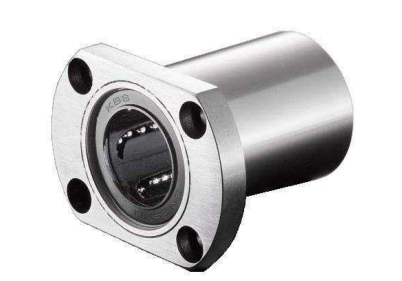
\includegraphics[width=\textwidth]{zhou6.png}
          \caption{直线轴承}
  \end{subfigure}
  \quad
  \begin{subfigure}[b]{0.35\textwidth}
          \centering
          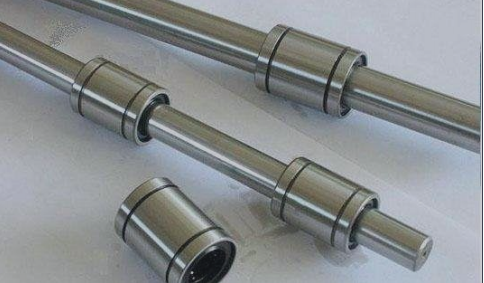
\includegraphics[width=\textwidth]{zhou7.png}
          \caption{直线轴承与轴}
  \end{subfigure}
  \caption{直线轴承示意图}
\end{figure}

\subsection{交叉滚子轴承}
交叉滚子轴承是一种内圈分割、外圈旋转 的特殊型号轴承。因被分割的内环或外环,在装入滚柱和间隔保持器后,与交叉滚柱轴环固定在一起,以防止互相分离,故安装交叉滚柱轴环时操作简单。由于滚柱为交叉排列,因此只用1套交叉滚柱轴环就可承受各个方向的负荷,与传统型号相比,刚性提高3~4倍。同时,因交叉滚子轴承内圈或外圈是两分割的构造,轴承间隙可调整,即使被施加预载,也能获得高精度地旋转运动。而且,由于其特殊的结构,在工业机器人中通常用作关节轴承。在RM比赛中,由于交叉滚子轴承优秀的性能,常用于云台yaw轴结构。

\begin{figure}[h]
  \centering
  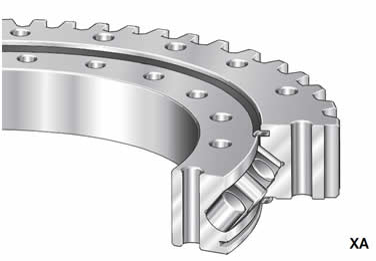
\includegraphics[width=0.3\textwidth]{zhou8.png}
  \caption{交叉滚子轴承示意图}
\end{figure}

\subsection{关节轴承}
关节轴承的结构比滚动轴承简单,其主要是由一个有外球面的内圈和一个有内球面的外圈组成。关节轴承一般用于速度较低的摆动运动(即角运动),由于滑动表面为球面形,亦可在一定角度范围内作倾斜运动(即调心运动),在支承轴与轴壳孔不同心度较大时,仍能正常工作。自润滑关节轴承应用于水利、专业机械等行业。关节轴承一般分为向心关节轴承和杆端关节轴承。

\begin{figure}[h]
  \centering
  \includegraphics[width=0.4\textwidth]{zhou9.png}
  \caption{关节轴承示意图}
\end{figure}

\section{弹簧}

弹簧是一种利用弹性来工作的机械零件。用弹性材料制成的零件在外力作用下发生形变,除去外力后又恢复原状。亦作“ 弹簧 ”。一般用弹簧钢制成。弹簧的种类复杂多样,按形状分,主要有螺旋弹簧、涡卷弹簧、板弹簧、异型弹簧等。

\begin{figure}[h]
  \centering
  \includegraphics[width=0.3\textwidth]{th1.png}
  \caption{弹簧}
\end{figure}

\subsection{压缩弹簧}
压缩弹簧(压簧)是承受轴向压力的螺旋弹簧,弹簧一般分为等节距弹簧和变节距弹簧,压缩弹簧的形状有:圆柱形、圆锥形、中凸形和中凹形以及少量的非圆形等,压缩弹簧的圈与圈之间有一定的间隙,当受到外载荷时弹簧收缩变形,储存变形能。变节距的弹簧越来越普遍,不在是只是等节距弹簧,变节距弹簧能够在不同的环境下发挥出不同的作用。

\begin{figure}[h]
  \centering
  \includegraphics[width=0.3\textwidth]{th2.png}
  \caption{压缩弹簧}
\end{figure}

压缩弹簧弹力的计算公式:$k=\frac{Gd^4}{8nD^3}$
上面公式里每项代表的含义为:
1、$G$ : 剪切弹性模量$[MPa, psi]$($G$值大小为:钢丝8000,不锈钢7200);
2、$d$ : 线径 $[mm, in]$;
3、$n$ : 有效圈数 $[-]$;
4、$D$ : 中心直径 $[mm]$;
5、$k$ : 弹簧系数 $[N/mm]$.



\subsection{拉伸弹簧}
拉伸弹簧(拉簧)是承受轴向拉力的螺旋弹簧,拉伸弹簧一般都用圆截面材料制造。在不承受负荷时,拉伸弹簧的圈 与圈之间一般都是并紧的没有间隙。利用拉伸后的回弹力(拉力)工作,用以控制机件的运动、贮蓄能量、测量力的大小等,广泛用于机器、仪表中。

\begin{figure}[h]
  \centering
  \includegraphics[width=0.3\textwidth]{tan3.png}
  \caption{拉伸弹簧}
\end{figure}

\subsection{扭力弹簧}
扭力弹簧(扭簧)利用杠杆的原理,通过对材质柔软、韧度较大的弹性材料的扭曲或旋转,使之具有极大的机械能。是承受扭转变形的弹簧,它的工作部分也是各圈或是紧密围绕或是分开围绕。扭转弹簧的端部结构是加工成各种形状的扭臂,由单扭至双扭,乃至各种扭杆之变形,得依设计成型。扭转弹簧常用于机械中的平衡机构,在汽车、机床、电器等工业生产中广泛应用。

\begin{figure}[h]
  \centering
  \includegraphics[width=0.3\textwidth]{th.png}
  \caption{扭力弹簧}
\end{figure}


\subsection{片弹簧}
片弹簧是利用弹性金属片的变形而产生弹簧特性的一种最简便的弹簧。弹性金属片有矩形、梯形、三角形,也可为直片、弯片。通常用于载荷和变形较小、要求刚度不大的地方,如仪器、仪表及自动化机构中的敏感元件、弹性支承或定位装置中。如电器通断触点等。

\begin{figure}[h]
  \centering
  \includegraphics[width=0.3\textwidth]{th3.png}
  \caption{片弹簧}
\end{figure}


\subsection{发条弹簧}
发条簧又名(卷)弹簧 ,是指螺旋线在一个平面内的弹簧,弹簧是将材料绕制成平面螺旋形的一种弹簧,弹簧一端固定,另一端作用扭矩后材料材料受弯曲力矩,产生弯曲弹性变形,因而弹簧在自身平面产生扭转。其变形角的大小和扭矩成正比,具有高扭力,与多角度之扭转力距故运用于长时间作功之机构,具有不易疲劳的特性,其运用类似扭簧。

\begin{figure}[h]
  \centering
  \includegraphics[width=0.3\textwidth]{th4.png}
  \caption{发条弹簧}
\end{figure}



\section{驱动元件}

\subsection{气动元件}
气动简介:气动是利用撞击作用或转动作用产生的空气压力使其运动或作功,\textbf{气动就是以压缩空气为动力源,带动机械完成伸缩或旋转动作}。因为是利用空气具有压缩性的特点,吸入空气压缩储存,空气便像弹簧一样具有了弹力,然后用控制元件控制其方向,带动执行元件的旋转与伸缩。RM比赛使用的气动系统大致可以分为三个部分:气源部分;控制部分;执行部分。

\begin{figure}[h]
  \centering
  \includegraphics[width=0.3\textwidth]{qi1.png}
  \caption{气动驱动系统}
\end{figure}

\begin{enumerate}
  \item \textbf{气源:} 
  气源,即提供压缩气体的装置。比赛使用的气源由气瓶和减压阀构成。气瓶提供压缩气体,减压阀使输出气压恒定。
  \begin{itemize}
    \item \textbf{气瓶:}气瓶是指在正常环境温度$(-40 \sim 60^{\circ}C)$ 下可重复充气使用的移动式压力容器。比赛使用气瓶为一般为钢制气瓶,可承受30Mp的压力,用于容纳压缩气体。气瓶一般为钢制,也有碳纤维气瓶,用于需要减重的场合。
    
    \begin{figure}[h]
      \centering
      \includegraphics[width=0.3\textwidth]{qi2.png}
      \caption{气瓶}
    \end{figure}

    \item \textbf{减压阀:}减压阀是通过调节,将进口压力减至某一需要的出口压力,并依靠介质本身的能量,使出口压力自动保持稳定的阀门。通过减压阀可以实现输出气压恒定,比赛使用气压一般为$1MPa$。

    \begin{figure}[h]
      \centering
      \includegraphics[width=0.3\textwidth]{qi3.png}
      \caption{减压阀}
    \end{figure}

  \end{itemize}
  \item \textbf{电磁阀(控制元件):} 电磁阀(Electromagnetic valve)是用电磁控制的工业设备,是用来控制流体的自动化基础元件,属于执行器,并不限于液压、气动。用在工业控制系统中调整介质的方向、流量、速度和其他的参数。电磁阀可以配合不同的电路来实现预期的控制,而控制的精度和灵活性都能够保证。电磁阀有很多种,不同的电磁阀在控制系统的不同位置发挥作用,最常用的是单向阀、安全阀、方向控制阀、速度调节阀等。
  
  电磁阀里有密闭的腔,在不同位置开有通孔,每个孔连接不同的油管,腔中间是活塞,两面是两块电磁铁,哪面的磁铁线圈通电阀体就会被吸引到哪边,通过控制阀体的移动来开启或关闭不同的排油孔,而进油孔是常开的,液压油就会进入不同的排油管,然后通过油的压力来推动油缸的活塞,活塞又带动活塞杆,活塞杆带动机械装置。这样通过控制电磁铁的电流通断就控制了机械运动。

  \begin{figure}[H]
    \centering
    \begin{subfigure}[b]{0.4\textwidth}
           \centering
           \includegraphics[width=\textwidth]{qi4.png}
            \caption{电磁阀}
    \end{subfigure}
    \quad
    \begin{subfigure}[b]{0.3\textwidth}
            \centering
            \includegraphics[width=\textwidth]{qi5.png}
            \caption{电磁阀原理图}
    \end{subfigure}
  \end{figure}

  \item \textbf{气缸(气动执行元件):} \textbf{气压传动中将压缩气体的压力能转换为机械能的气动执行元件。}气缸有做往复直线运动的和做往复摆动两种类型(见图)。做往复直线运动的气缸又可分为单作用气缸、双作用气缸、膜片式气缸和冲击气缸4种。\textbf{比赛一般使用双作用气缸}(双作用气缸:从活塞两侧交替供气,在一个或两个方向输出力。)

  \begin{figure}[H]
    \centering
    \begin{subfigure}[b]{0.4\textwidth}
           \centering
           \includegraphics[width=\textwidth]{qi6.png}
            \caption{气缸}
    \end{subfigure}
    \quad
    \begin{subfigure}[b]{0.37\textwidth}
            \centering
            \includegraphics[width=\textwidth]{qi7.png}
            \caption{气缸原理图}
    \end{subfigure}
  \end{figure}

\end{enumerate}

\subsection{电机}
电机的主要作用是产生驱动转矩,作为用电器或各种机械的动力源。按用途可划分:驱动用电动机和控制用电动机。控制用电动机又划分:步进电动机和伺服电动机等。

驱动用电动机主要用于提供驱动力,可划分:电动工具(包括钻孔、抛光、磨光、开槽、切割、扩孔等工具)用电动机、家电(包括洗衣机、电风扇、电冰箱、空调器、录音机、录像机、影碟机、吸尘器、照相机、电吹风、电动剃须刀等)用电动机及其他通用小型机械设备(包括各种小型机床、小型机械、医疗器械、电子仪器等)用电动机。

控制用电动机可以精确控制旋转角度,又划分:步进电动机和伺服电动机等,接下来各章会介绍RM比赛电机。

\begin{figure}[H]
  \centering
  \begin{subfigure}[b]{0.3\textwidth}
         \centering
         \includegraphics[width=\textwidth]{dj1.png}
          \caption{步进电机}
  \end{subfigure}
  \quad
  \begin{subfigure}[b]{0.22\textwidth}
          \centering
          \includegraphics[width=\textwidth]{dj2.png}
          \caption{伺服电机}
  \end{subfigure}
\end{figure}

\subsubsection{常用电机参数}
\begin{enumerate}
  \item \textbf{标称功率或额定功率:} 指电机系统工设计时的工作能力的重要指标。理想功率也是在推荐工作情况下的最大功率。额定功率是表征电机性能的重要指标。
  \item \textbf{额定电压或工作电压:} 由于一般电机可以工作在不同电压下,但电压直接和转速有关,其他参数也相应变化,所以该电压只是一种建议电压,其他参数也是在这种推荐的电压下给出的。
  \item \textbf{空载转速:} 单位RPM(转/分钟),即每分钟多少转。
  \item \textbf{额定转速:} 在额定功率下的电机转速。也即满载下的电机转速。
  \item \textbf{堵转扭矩:}此参数是很多带负载电机的重要参数。即在电机受反向外力使其停止转动时的力矩。如果电机堵转现象经常出现,则会损坏电机,或烧坏驱动芯片,所以大家选电机时,这是除转速外第一个考虑的参数。不过需注意,堵转时间一长,电机温度上升很快,这个值也会迅速下降。
  \item \textbf{额定转矩:} 转矩是一种力矩,力矩定义是:力矩$ = $力 $ \times $ 力臂。这里力臂可以看成电机所带动的物体的转动半径。如果力矩太小,就带不动所要带动的物体,也就是感觉电机“劲”不够大。
  \item \textbf{空载电流或空转电流:} 空载电流和电压的乘积形成的能量,主要分为势能和热能消耗。热能就是电机线圈的发热,越好的电机,在空载时,该值越小;而势能指克服摩擦力,和转子自身惯性的能量还有转子自身的转动势能。而一般转速一定时,转子的惯性能量增加几乎没有,而这个势能主要还是克服摩擦力的问题,而最终以热能形式耗散。所以空载电流越小,电机性能越好,特别是加上减速箱的电机,空载电流越小,说明减速箱做的越好,当然,减速比越大,同样的设计方式下,阻力越大。
  \item \textbf{额定电流:} 在额定电压下,额定功率状态下的电机工作电流。
  \item \textbf{起动电流:} 电机在额定电压下,额定频率下起动时的电流。一般数倍于额定电流。大的起动电流会引起电力网电压波动,影响用电设备的正常使用。这个参数也比较重要。转子的惯量在这更加体现。好的电机,在同样加速度下,起动电流较小。
  \item \textbf{最大转速或最大允许转速:}最大转速就是不考虑扭矩和功率输出,可以实现的电机最大输出转速。这个参数对于表征速度范围和控制器的设计匹配有用。
  \item \textbf{最大连续电流:} 这个电流主要指有反向外力时,比如有负载时出现的电流。一般这个电流和电压乘积小于额定功率,并不是说该电机就是有一个损耗比,而是长时间在大电流情况下工作如额定功率下,会导致温度升高,直接后果就是电阻增加,效率下降,并导致整体性能下降,而且有可能损坏设备。在这个值下工作,一般就可以保证长时间正常运转。
  \item \textbf{最大连续转矩:} 与最大连续电流的作用概率类似
  \item \textbf{最大输出功率:} 额定电压下最大输出功率。与额定功率的区别在于这个功率不考虑安全性,不是能长时间保持的值。
  \item \textbf{电机效率:}电机效率指的是:电机消耗的电能与转换成机械动能之比。例如电机消耗的电能是3000瓦,而产生的机械动能是2700瓦,其效率就是$90\%$
  \item \textbf{转子惯量:} 也称转子转动惯量,转动惯量是刚体绕轴转动时惯性的量度。
\end{enumerate}


\subsubsection{M3508减速电机}
\textbf{M3508电机是比赛最为常用的驱动电机},配备定制FOC电调(C620电机调速器),\textbf{可广泛应用于机器人移动平台动力、驱动模块等}。

M3508减速电机套装最大功率高达220W,最大扭矩$5N \cdot m$;最大持续功率$150W$,持续扭矩$2.8N \cdot m$,有感FOC控制不论转速高低都能提供稳定的扭矩,让机器人在快速响应的同时保持平稳的动力。

\begin{figure}[H]
  \centering
  \begin{subfigure}[b]{0.4\textwidth}
         \centering
         \includegraphics[width=\textwidth]{dj3.png}
          \caption{M3508电机和C620电调}
  \end{subfigure}
  \quad
  \begin{subfigure}[b]{0.34\textwidth}
          \centering
          \includegraphics[width=\textwidth]{dj4.png}
          \caption{M3508电机组成的移动平台动力系统}
  \end{subfigure}
  \caption{M3508减速电机}
\end{figure}

\subsubsection{M2006动力系统}
RoboMaster M2006动力系统由RoboMaster M2006 P36直流无刷减速电机和RoboMaster C610无刷电机调速器组成,具有控制精度高,输出功率大,体积小等特性。相比于RoboMaster M3508动力系统,转速接近,体积和重量大幅下降。

\begin{figure}[H]
  \centering
  \begin{subfigure}[b]{0.35\textwidth}
         \centering
         \includegraphics[width=\textwidth]{dj5.png}
          \caption{M2006电机和C610电调}
  \end{subfigure}
  \quad
  \begin{subfigure}[b]{0.39\textwidth}
          \centering
          \includegraphics[width=\textwidth]{dj6.png}
          \caption{M2006电机组成的移动平台动力系统}
  \end{subfigure}
  \caption{M2006减速电机}
\end{figure}

\subsubsection{GM6020动力系统}
RoboMaster GM6020 是一款内部集成驱动器的高性能\textbf{直流无刷电机}。电机采用\textbf{空心轴设计},扭矩密度大、\textbf{控制精度高}、交互方式灵活、保护功能强,适用于低转速、大扭矩直接驱动的应用场景,是机器人比赛、科研教育、自动化设备等领域的理想之选,\textbf{RM比赛当中常作为云台电机使用}。

\begin{figure}[H]
  \centering
  \begin{subfigure}[b]{0.4\textwidth}
         \centering
         \includegraphics[width=\textwidth]{dj7.png}
          \caption{GM6020电机}
  \end{subfigure}
  \quad
  \begin{subfigure}[b]{0.39\textwidth}
          \centering
          \includegraphics[width=\textwidth]{dj8.png}
          \caption{GM6020电机尺寸图}
  \end{subfigure}
  \caption{GM6020电机}
\end{figure}

\textbf{电机安装:} 电机安装板的设计一般要考虑三个方面。

\begin{enumerate}
  \item \textbf{定位孔:}定位孔一般用于保证同轴度。电机安装面上一般都一圆形凸台结构,定位孔尺寸与该凸台一致,安装是孔与凸台紧配合,从而保证同心;
  \item \textbf{安装孔:}用于安装螺栓的孔位;
  \item \textbf{指示灯、拨码开关、线头等:}这一点要根据具体情况确定,安装结构不能遮挡指示灯,线头,拨码开关等需要经常使用的部位。
\end{enumerate}

\begin{figure}[H]
  \centering
  \begin{subfigure}[b]{0.4\textwidth}
         \centering
         \includegraphics[width=\textwidth]{an1.png}
          \caption{GM6020电机尺寸图}
  \end{subfigure}
  \quad
  \begin{subfigure}[b]{0.4\textwidth}
          \centering
          \includegraphics[width=\textwidth]{an2.png}
          \caption{电机安装板实例图}
  \end{subfigure}
  \caption{GM6020电机安装示意图}
\end{figure}


\subsection{舵机}

舵机是一种位置(角度)伺服的驱动器。舵机主要适用于那些需要角度不断变化并可以保持的控制系统,比如人形机器人的手臂和腿,车模和航模的方向控制。舵机的控制信号实际上是一个脉冲宽度调制信号(PWM信号),该信号可由FP-GA器件、模拟电路或单片机产生。

厂商所提供的舵机规格资料,都会包含外形尺寸$(mm)$、扭力$(kg \cdot cm)$、速度$(s/60^{\circ})$、测试电压$(V)$及重量$(g)$等基本资料。扭力的单位是$kg \cdot cm$,意思是在摆臂长度 $1cm$处,能吊起几公斤重的物体。这就是力臂的观念,因此摆臂长度愈长,则扭力愈小。速度的单位是 $sec/60^{\circ}$,意思是舵机转动$60^{\circ}$所需要的时间。

\begin{figure}[H]
  \centering
  \begin{subfigure}[b]{0.4\textwidth}
         \centering
         \includegraphics[width=\textwidth]{duo1.png}
          \caption{舵机和舵盘}
  \end{subfigure}
  \quad
  \begin{subfigure}[b]{0.28\textwidth}
          \centering
          \includegraphics[width=\textwidth]{duo2.png}
          \caption{舵机和舵机支架}
  \end{subfigure}
  \caption{舵机示意图}
\end{figure}

\section{传动零件}
传动是指机械之间的动力传递,也可以说将机械动力通过中间媒介传递给终端设备,这种传动方式包括链条传动、摩擦传动、液压传动、齿轮传动以及皮带式传动等,下面将从常用的几种传动方式进行介绍。

\subsection{同步带}
同步带传动通过传动带内表面上等距分布的横向齿和带轮上的相应齿槽的啮合来传递运动。与摩擦型带传动比较,\textbf{同步带传动的带轮和传动带之间没有相对滑动,能够保证严格的传动比}。但同步带传动对中心距及其尺寸稳定性要求较高,\textbf{一般需要张紧轮或腰形孔辅助张紧}。

\begin{figure}[H]
  \centering
  \begin{subfigure}[b]{0.4\textwidth}
         \centering
         \includegraphics[width=\textwidth]{tb1.png}
          \caption{同步带轮}
  \end{subfigure}
  \quad
  \begin{subfigure}[b]{0.4\textwidth}
          \centering
          \includegraphics[width=\textwidth]{tb2.png}
          \caption{同步带传动}
  \end{subfigure}
  \caption{同步带传动示意图}
\end{figure}

同步带传动优点 :
\begin{itemize}
  \item 传动准确,工作时无滑动,具有恒定的传动比;
	\item 传动平稳,具有缓冲、减振能力,噪声低;
	\item 传动效率高,可达 0.98,节能效果明显;
	\item 维护保养方便,不需润滑,维护费用低;
	\item 速比范围大,一般可达 10,线速度可达 $50m/s$,有较大的功率传递范围,可达几瓦到几百千瓦;
	\item 可用于长距离传动,中心距可达 $10m$ 以上。
\end{itemize}
	
\subsection{链轮链条}
\textbf{链轮传动简介:}链传动是通过链条将具有特殊齿形的主动链轮的运动和动力传递到具有特殊齿形的从动链轮的一种传动方式。
\textbf{链轮传动优点:}与带传动相比,无弹性滑动和打滑现象,平均传动比准确,工作可靠,效率高;\textbf{传递功率大,过载能力强},相同工况下的传动尺寸小;所需张紧力小,作用于轴上的压力小;能在高温、潮湿、多尘、有污染等恶劣环境中工作。
\textbf{链轮传动缺点:}仅能用于两平行轴间的传动;成本高,易磨损,易伸长,传动平稳性差,运转时会产生附加动载荷、振动、冲击和噪声,\textbf{不宜用在急速反向的传动中}。

\begin{figure}[H]
  \centering
  \begin{subfigure}[b]{0.4\textwidth}
         \centering
         \includegraphics[width=\textwidth]{ll1.png}
          \caption{链轮传动}
  \end{subfigure}
  \quad
  \begin{subfigure}[b]{0.3\textwidth}
          \centering
          \includegraphics[width=\textwidth]{ll2.png}
          \caption{链轮}
  \end{subfigure}
  \caption{链轮传动示意图}
\end{figure}

\subsection{滚珠丝杆}
\textbf{滚珠丝杠是将回转运动转化为直线运动,或将直线运动转化为回转运动的理想的产品。}滚珠丝杠是工具机械和精密机械上最常使用的传动元件,其主要功能是将旋转运动转换成线性运动,或将扭矩转换成轴向反复作用力,同时兼具高精度、可逆性和高效率的特点。由于具有很小的摩擦阻力,滚珠丝杠被广泛应用于各种工业设备和精密仪器。
滚珠丝杠由螺杆、螺母、钢球、预压片、反向器、防尘器组成。它的功能是将旋转运动转化成直线运动,这是艾克姆螺杆的进一步延伸和发展,这项发展的重要意义就是将轴承从滑动动作变成滚动动作。

\begin{figure}[H]
  \centering
  \begin{subfigure}[b]{0.35\textwidth}
         \centering
         \includegraphics[width=\textwidth]{g1.png}
          \caption{单轴滚珠丝杠}
  \end{subfigure}
  \quad
  \begin{subfigure}[b]{0.4\textwidth}
          \centering
          \includegraphics[width=\textwidth]{g2.png}
          \caption{双轴滚珠丝杠}
  \end{subfigure}
  \caption{滚珠丝杠示意图}
\end{figure}

\subsection{齿轮传动}
\textbf{齿轮传动简介 :}齿轮传动是指由齿轮副传递运动和动力的装置,它是现代各种设备中应用最广泛的一种机械传动方式。它的传动比较准确,效率高,结构紧凑,工作可靠,寿命长。

\textbf{齿轮参数:} 下面仅列举一些较为重要的齿轮参数。
\begin{itemize}
  \item \textbf{齿数Z:} 其中小齿轮齿数z1,大齿轮齿数z2。为了提高传动的平稳性,减小冲击振动,以齿数多一些为好,一般z1不小于17。
  \item \textbf{模数m:} 模数是指相邻两轮齿同侧齿廓间的齿距p与圆周率π的比值(m=p/π),以毫米为单位。模数是模数制轮齿的一个最基本参数。模数m决定齿轮尺寸,齿数相同的齿轮模数大,则其尺寸也大。
  \item \textbf{分度圆直径:} $d=m*z$
  \item \textbf{中心距:} $a=\frac{1}{2}m(z_1+z_2)$
\end{itemize}

\begin{figure}[H]
  \centering
  \begin{subfigure}[b]{0.4\textwidth}
         \centering
         \includegraphics[width=\textwidth]{cl1.jpg}
          \caption{齿轮}
  \end{subfigure}
  \quad
  \begin{subfigure}[b]{0.33\textwidth}
          \centering
          \includegraphics[width=\textwidth]{cl2.png}
          \caption{齿轮参数}
  \end{subfigure}
  \caption{齿轮示意图}
\end{figure}

齿轮按其外形分为圆柱齿轮、锥齿轮、非圆齿轮、齿条、蜗杆蜗轮;按齿线形状分为直齿轮、斜齿轮、人字齿轮、曲线齿轮,下面是部分齿轮传动的示意图。

\begin{figure}[h]
  \centering
  \includegraphics[width=0.5\textwidth]{cl3.png}
  \caption{各种齿轮啮合示意图}
\end{figure}

\section{其他}
除上述零件外,还有些其他零件供大家参考。
\subsection{卡簧}
卡簧简介:卡簧,也叫挡圈或扣环,属于紧固件的一种,供装在机器、设备的轴槽或孔槽中,起着阻止轴上或孔上的零件轴向运动的作用,分为轴用卡簧和孔用卡簧。

\begin{figure}[h]
  \centering
  \includegraphics[width=0.5\textwidth]{ka.png}
  \caption{卡簧,轴用卡簧(左)孔用卡簧(右)}
\end{figure}

卡簧安装:卡簧钳,拆装卡簧的专用工具。卡簧钳有孔用和轴用两种。卡簧取出或者安装时,使用的专用工具常态时钳口打开的是孔用卡簧钳;常态时钳口闭合的是轴用卡簧钳。

\begin{figure}[H]
  \centering
  \begin{subfigure}[b]{0.4\textwidth}
         \centering
         \includegraphics[width=\textwidth]{ka1.png}
          \caption{卡簧钳}
  \end{subfigure}
  \quad
  \begin{subfigure}[b]{0.2\textwidth}
          \centering
          \includegraphics[width=\textwidth]{ka2.png}
          \caption{卡簧安装示意图}
  \end{subfigure}
\end{figure}



\subsection{铜柱,铝柱,尼龙柱}
六角铜柱,头部一般带有螺纹孔或螺栓头,用于构成支撑结构。根据头部类型可分为双通六角铜柱,单头六角铜柱等。另外,与铜柱作用相似还有铝柱,尼龙柱等,使用材料不同但用法完全一致,尼龙柱质量最轻同样强度最低,铝柱以及铜柱强度较高,但铜柱比铝柱质量偏大,一般常用铝柱。

\begin{figure}[H]
  \centering
  \begin{subfigure}[b]{0.21\textwidth}
         \centering
         \includegraphics[width=\textwidth]{tong1.png}
          \caption{双通铜柱}
  \end{subfigure}
  \quad
  \begin{subfigure}[b]{0.21\textwidth}
          \centering
          \includegraphics[width=\textwidth]{tong2.png}
          \caption{单通铜柱}
  \end{subfigure}
  \quad
  \begin{subfigure}[b]{0.28\textwidth}
          \centering
          \includegraphics[width=\textwidth]{tong3.png}
          \caption{铜柱安装示意图}
  \end{subfigure}
  \caption{铜柱示意图}
\end{figure}

\subsection{滑块滑轨}
主要有滑块和导轨组成,滑块主要应用于滑动摩擦导轨。直线导轨又称线轨、滑轨、线性导轨、线性滑轨,用于直线往复运动场合,且可以承担一定的扭矩,可在高负载的情况下实现高精度的直线运动。

\textbf{直线导轨运动的作用是用来支撑和引导运动部件,按给定的方向做往复直线运动。}依按摩擦性质而定,直线运动导轨可以分为滑动摩擦导轨、滚动摩擦导轨、弹性摩擦导轨、流体摩擦导轨等种类。直线导轨主要是用在精度要求比较高的机械结构上,直线导轨的移动元件和固定元件之间不用中间介质,而用滚动钢球。

\begin{figure}[h]
  \centering
  \includegraphics[width=0.3\textwidth]{hua.png}
  \caption{滑块滑轨}
\end{figure}

\section{结语}
该培训手册只是对机械结构设计常用的零件做一个科普性的介绍。如果要深入了解,最好自行查询相关资料。图\ref{jxs}所示为机械设计手册,主要供机械设计者查询使用。本书全面系统地介绍了常规设计、机电一体化与控制技术和现代设计方法及其应用等内容。具有内容先进、信息量大、取材广、规格全,实用性强,数据可靠,使用方便等特点。全书分6卷52篇,内容有:常用设计资料、机械零部件设计(连接、紧固与传动)、机械零部件设计(轴系、支承与其他)、流体传动与控制、机电一体化及控制技术、现代设计理论与方法等\cite{bai}。

\begin{figure}[h]
  \centering
  \includegraphics[width=0.3\textwidth]{jx.png}
  \caption{机械设计手册}
  \label{jxs}
\end{figure}

最后,机械结构设计能力需要在实践当中提升,尤其是对各种结构性能的把握,只有足够的经验积累,才能在设计当中游刃有余的使用。

\bibliographystyle{unsrt}
\bibliography{myreff} 

\end{document}